\begin{figure}[t]
    \centering
    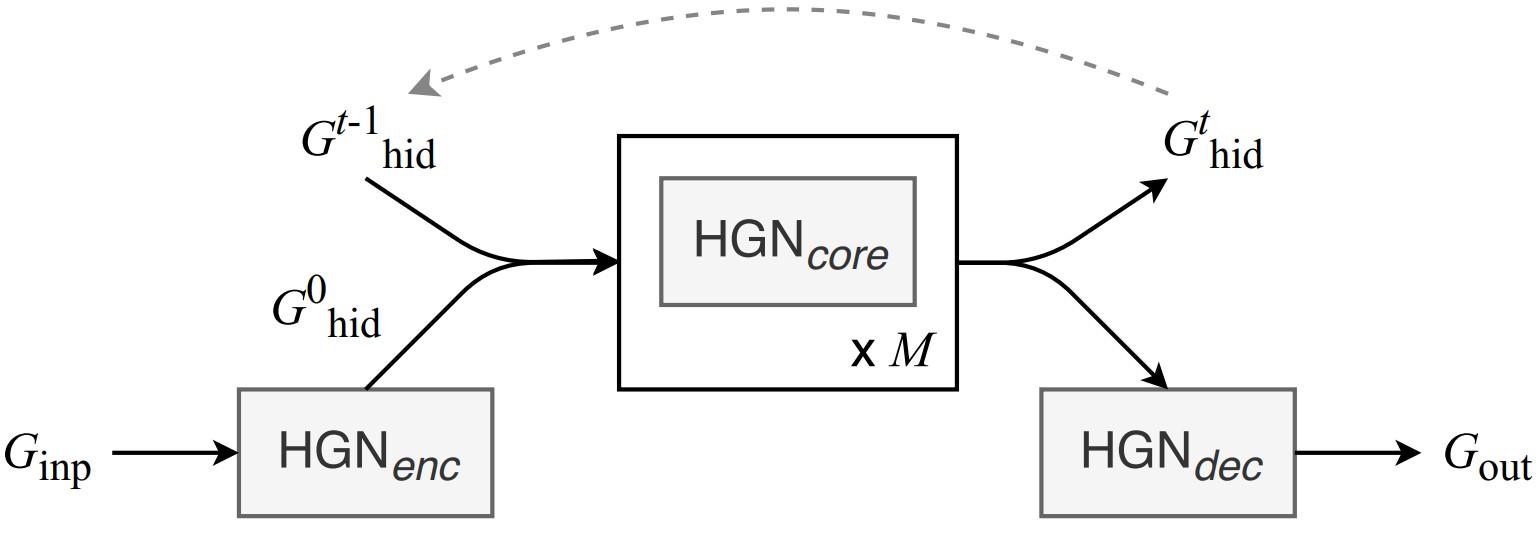
\includegraphics[width=0.8\textwidth]{figures/images/ch4/strips_hgn_architecture.jpg}
    \caption{Architecture of the STRIPS-HGN model \cite{shen2020learning}. The model is composed of three main components: the encoder, the hyper-graph network, and the decoder. The encoder processes the input graph, generating a first hidden graph representation. The HGN implements the message passing mechanism, updating the hidden graph representation. The decoder generates the output graph, which global value represents the predicted heuristic.}
    \label{fig:strips_hgn_architecture}
\end{figure}
